\section{Results}

\subsection{Dataset}
To test the already discussed data generation pipeline and deep learning models, we try to map the second floor of the Povo 1 building in the University of Trento.
We filmed a single vertical video with a smartphone (model: OPPO reno 4 CPH2091) at 2160x3840px 30fps of the entire floor, avoiding moving objects and people. The frames have been extracted at 10fps, resulting in 1462 images for a total of 13.1 GB. COLMAP has been used to generate a sparse reconstruction map using the Poisson mesher, high quality, shared intrinsics, and simple\_radial camera model.
Due to COLMAP limitations, different runs have been necessary, since the final reconstruction was not good enough, especially in terms of closed-loop detection: \cref{fig:trajectory-colmap} shows the best achieved result that has been used.

Due to the models' backend implementation, input images of the model should be 224x224: for this reason, resizing and center cropping has been adopted. The final size of the processed dataset is 880.3 MB. Train, validation, and test datasets have equal size and have been generated using the $\mod{3}$ operation on the frame index: in this way, adjacent frames are included in different datasets.

\subsection{PoseNet}
Since several pre-trained models can be used as the PoseNet backend, in \cref{tab:mapnet-backends} we present a brief list of them with the respective mean absolute error in the test set: notice that all the PoseNets have been tested with a single final linear layer. Even if the overall trend is similar, it is possible to notice that ResNet-152 and EfficientNet-B7 obtain the best results: this is mainly due to the performance list showed on the ImageNet dataset in \cref{tab:backend-performance-imagenet}. In this case, it means that more parameters make the difference, but causes also drawbacks in model performances.

\begin{table}[htbp]
    \caption{PoseNet backend comparison}
    \begin{center}
        \begin{tabular}{lrrrr}
            \toprule
            {Model}         & \thead{Position                                              \\error} & \thead{Rotation\\error} & \thead{Total\\parameters} & \thead{Trainable\\parameters} \\
            \midrule
            GoogLeNet       & 0.781           & 0.119          & $\sim$ 7,000,000 & 3,591  \\
            ResNet-18       & 0.635           & 0.288          & 11,180,103       & 3,591  \\
            ResNet-34       & 0.632           & 0.223          & 21,288,263       & 3,591  \\
            ResNet-50       & 0.707           & 0.191          & 23,522,375       & 14,343 \\
            ResNet-152      & \textbf{0.594}  & 0.139          & 58,158,151       & 14,343 \\
            EfficientNet-B7 & 0.817           & \textbf{0.132} & 63,804,887       & 17,927 \\
            \bottomrule
        \end{tabular}
        \label{tab:posenet-backends}
    \end{center}
\end{table}

In addition, trying to obtain the best results, different loss functions have been tested in the \cref{eq:menet-loss}. Note that in case of $\alpha \neq 1$ and MSE, the training loss is not tractable (goes to infinity).
\begin{figure}[htbp]
    \begin{center}
        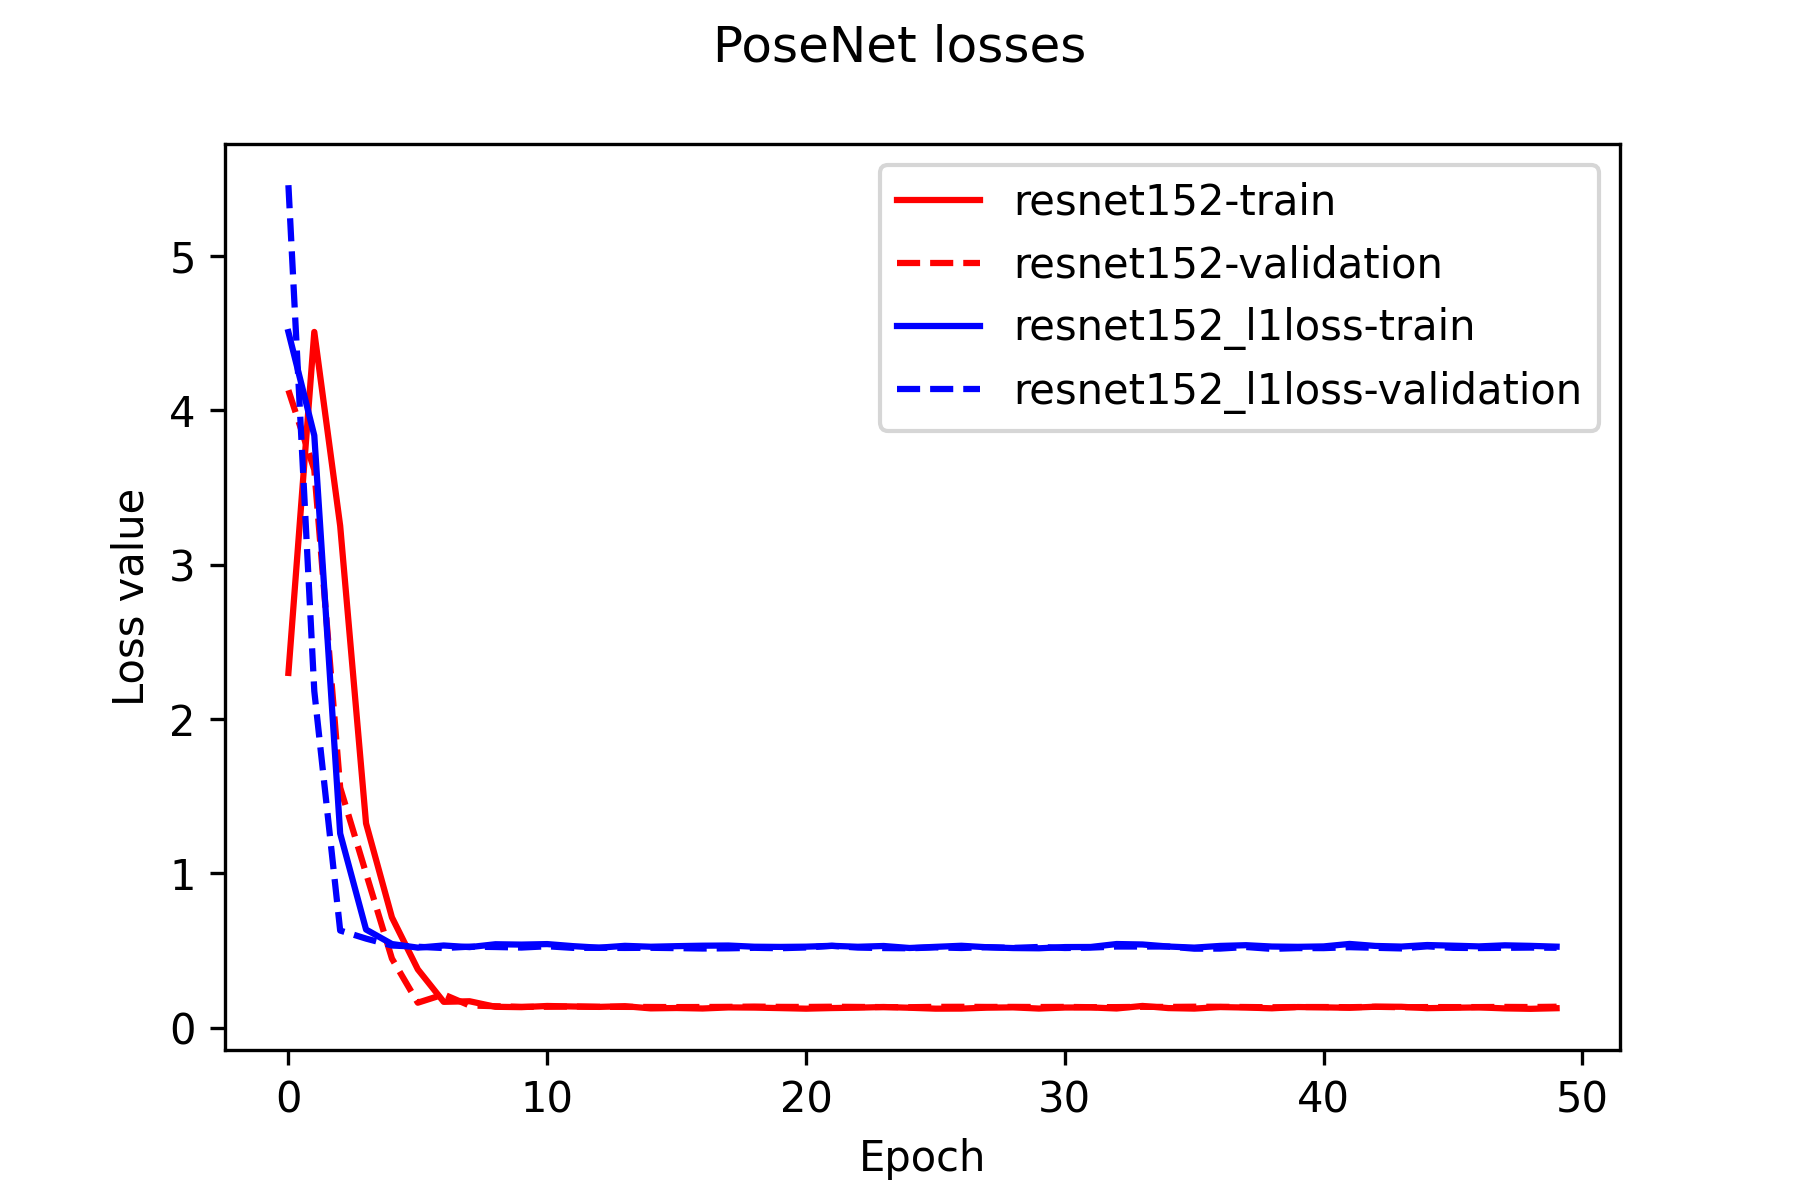
\includegraphics[width=0.4\textwidth]{./imgs/posenet_losses.png}
    \end{center}
    \caption{PoseNet (ResNet-152) losses.}
    \label{fig:posenet-losses}
\end{figure}

\Cref{fig:posenet-losses} shows the SmoothedL1Loss and L1Loss loss curves for a ResNet-152 PoseNet. It is possible to notice from \cref{tab:posenet-losses} that both in each of the two cases, the model is converging without overfitting.

\begin{table}[htbp]
    \caption{PoseNet losses comparison}
    \begin{center}
        \begin{tabular}{lrr}
            \toprule
            Loss            & {Position Error} & {Rotation Error} \\
            \midrule
            SmoothedL1Loss  & \textbf{0.594}   & \textbf{0.139}   \\
            L1Loss          & 0.906            & 0.226            \\
            MSE             & NaN              & NaN              \\
            $\alpha \neq 1$ & NaN              & NaN              \\
            \bottomrule
        \end{tabular}
        \label{tab:posenet-losses}
    \end{center}
\end{table}

\begin{figure*}[htbp]
    \begin{subfigure}[b]{0.48\textwidth}
        \centering
        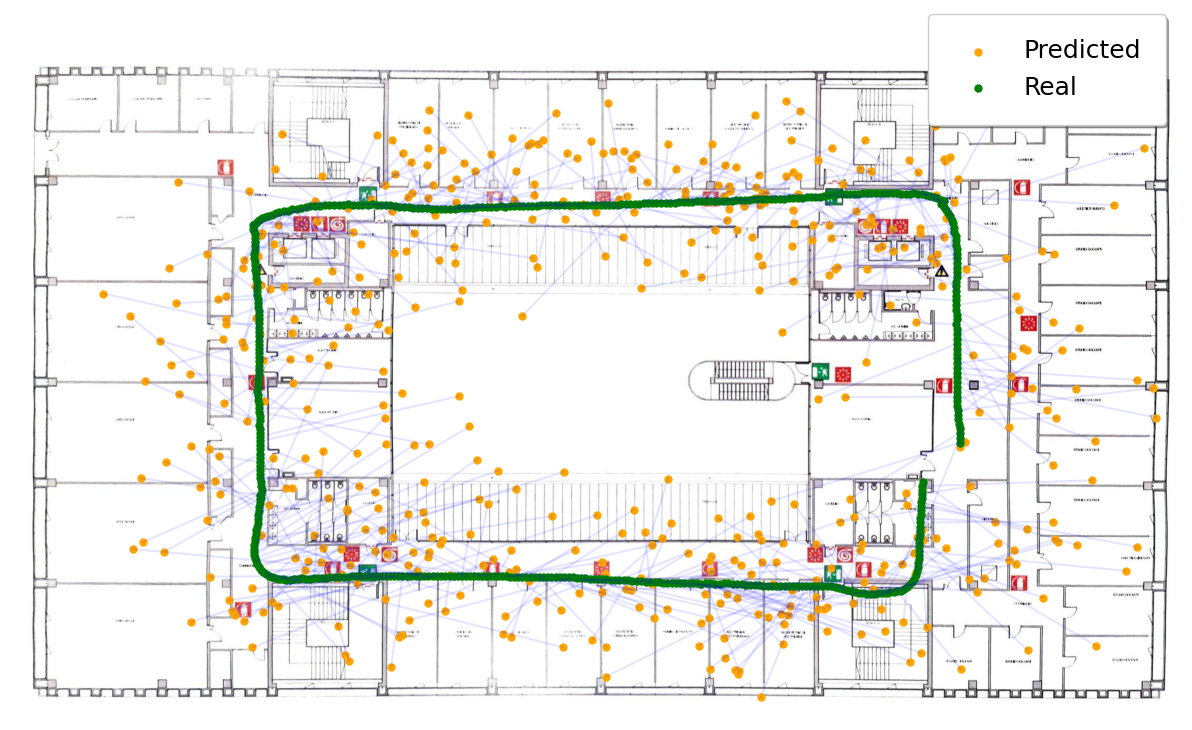
\includegraphics[width=1\textwidth]{./imgs/posenet_map.png}
        \caption{Predicted trajectory with PoseNet (ResNet-152).}
        \label{fig:trajectory-posenet}
    \end{subfigure}
    \hfill
    \begin{subfigure}[b]{0.48\textwidth}
        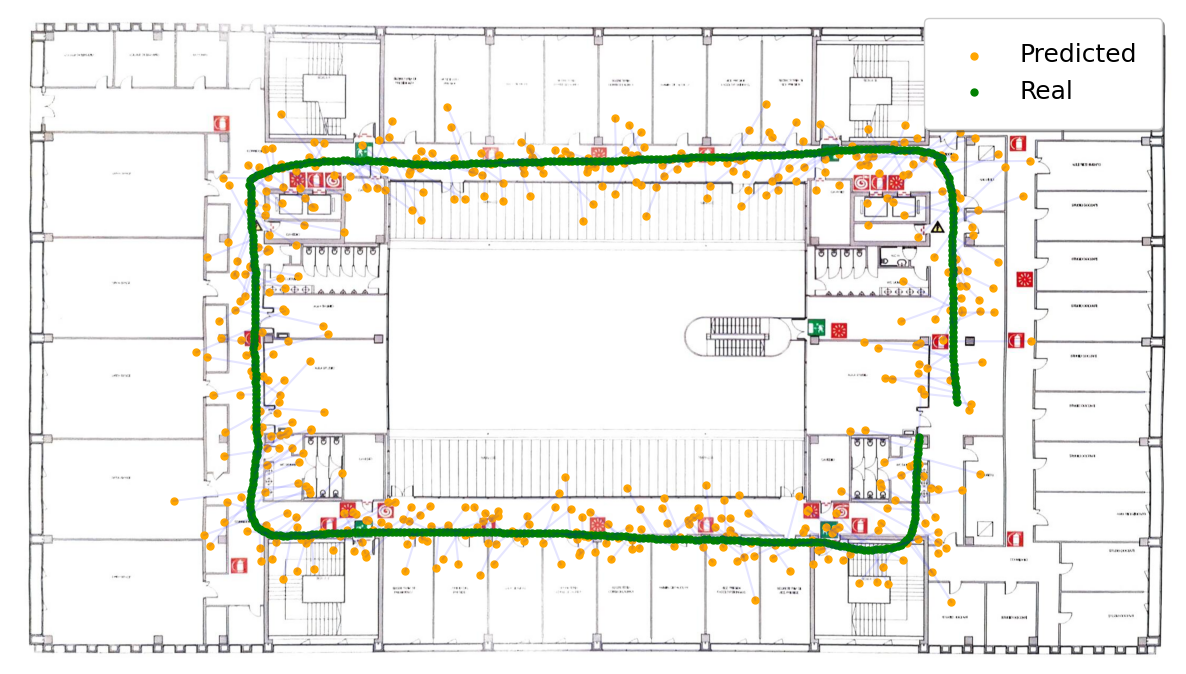
\includegraphics[width=1\textwidth]{./imgs/mapnet_map.png}
        \caption{Predicted trajectory MapNet (ResNet-34).}
        \label{fig:trajectory-mapnet}
    \end{subfigure}
    \caption{Estimated trajectories.}
\end{figure*}
\Cref{fig:trajectory-posenet} show a visual representation of the model performances. It is easy to notice that even if the predictions are almost in the same map zone with respect to their ground truth, they are still pretty sparse.

\subsection{MapNet}
To prevent sparsification in the model outputs, we propose the use of the MapNet. As for the PoseNet, also in this case several pre-trained models can be used as features extractor: \cref{tab:mapnet-backends} shows some candidates, each one used with three final linear layers.
In this case the overall trend is similar: this highlights that the extracted features are enough for the task independently of the backbone used. Another interesting difference with \cref{tab:posenet-backends} is the fact that models with more parameters are not the one performing better.
\begin{table}[htbp]
    \caption{MapNet backend comparison}
    \begin{center}
        \begin{tabular}{lrrrr}
            \toprule
            {Model}         & \thead{Position                                                  \\error} & \thead{Rotation\\error} & \thead{Total\\parameters} & \thead{Trainable\\parameters} \\
            \midrule
            GoogLeNet       & 0.225           & 0.0876          & $\sim$ 7,000,000 & 3,677,191 \\
            ResNet-18       & 0.202           & \textbf{0.0658} & 14,853,703       & 3,677,191 \\
            ResNet-34       & \textbf{0.187}  & 0.0757          & 24,961,863       & 3,677,191 \\
            ResNet-50       & 0.220           & 0.0969          & 30,330,951       & 6,822,919 \\
            ResNet-152      & 0.233           & 0.0869          & 64,966,727       & 3,677,191 \\
            EfficientNet-B7 & 0.210           & 0.0848          & 71,658,455       & 7,871,495 \\
            \bottomrule
        \end{tabular}
        \label{tab:mapnet-backends}
    \end{center}
\end{table}

Another interesting point is the importance of the final linear encoder, represented in terms of size with the number of trainable parameters in \cref{tab:posenet-backends,tab:mapnet-backends}. It is clear that more parameters are useful to better fit complex environments, so for this reason three linear layers have been used in our implementation with respect to the original one \cite{mapnet}.

Following the example of \cref{fig:posenet-losses} for the PoseNet model, \cref{fig:mapnet-losses} shows a comparison on the ResNet-34 MapNet for the training and validation curves for different losses. Also in this case the model is converging without overfitting.
\begin{figure}[htbp]
    \begin{center}
        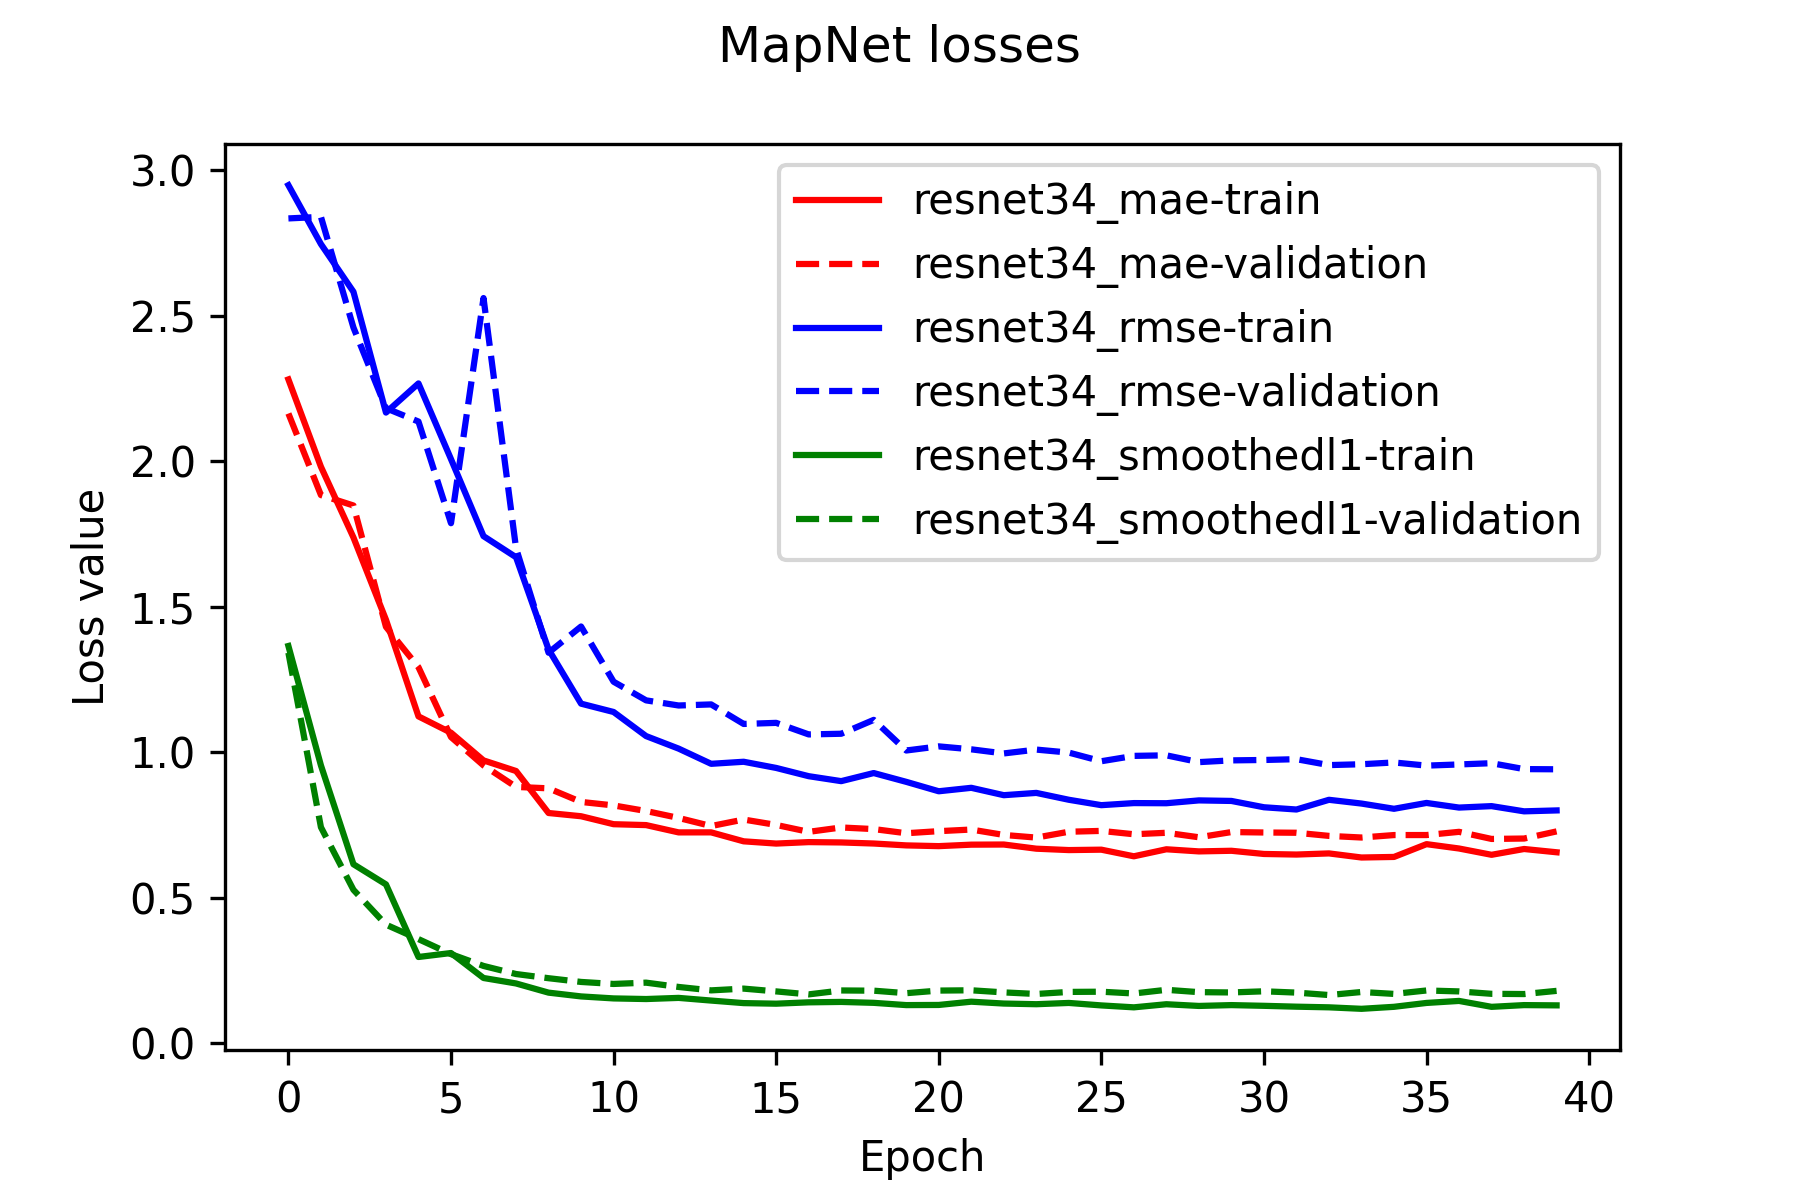
\includegraphics[width=0.4\textwidth]{./imgs/mapnet_losses.png}
    \end{center}
    \caption{MapNet (ResNet-34) losses}
    \label{fig:mapnet-losses}
\end{figure}

In this case, as can be seen in \cref{fig:trajectory-mapnet}, the custom MapNet predictions follow more closely the ground truth path with respect to the ones described by the PoseNet in \cref{fig:trajectory-posenet}.

Since this approach has been shown to still include some imperfections, we have also included a post-processing algorithm which tries to correct the model prediction. To be more specific, if the model prediction is not in a walkable spot in the map, then the output is going to be the nearest walkable point on the map according to the Euclidean distance criterion. The result can be viewed in \cref{fig:trajectory-mapnet-walkable}.

\subsection{Dashboard}
To be able to deploy the model, a web-server has been developed with FastAPI: this interface aims to easily allow users to interact with the production model through a web-based Bootstrap dashboard.
The dashboard can show the model predictions in three different ways:
\begin{itemize}
    \item raw model output which can be in a non-walkable zone displayed through an alert;
    \item raw model output which can be in a non-walkable zone shown in the floor map;
    \item post-processed model output in a walkable zone in the floor map.
\end{itemize}
\Cref{fig:dashboard} presents the \textit{UI} for showing post-precessed model outputs: red zones are not walkable areas.
\begin{figure*}[htbp]
    \begin{subfigure}[b]{0.542\textwidth}
        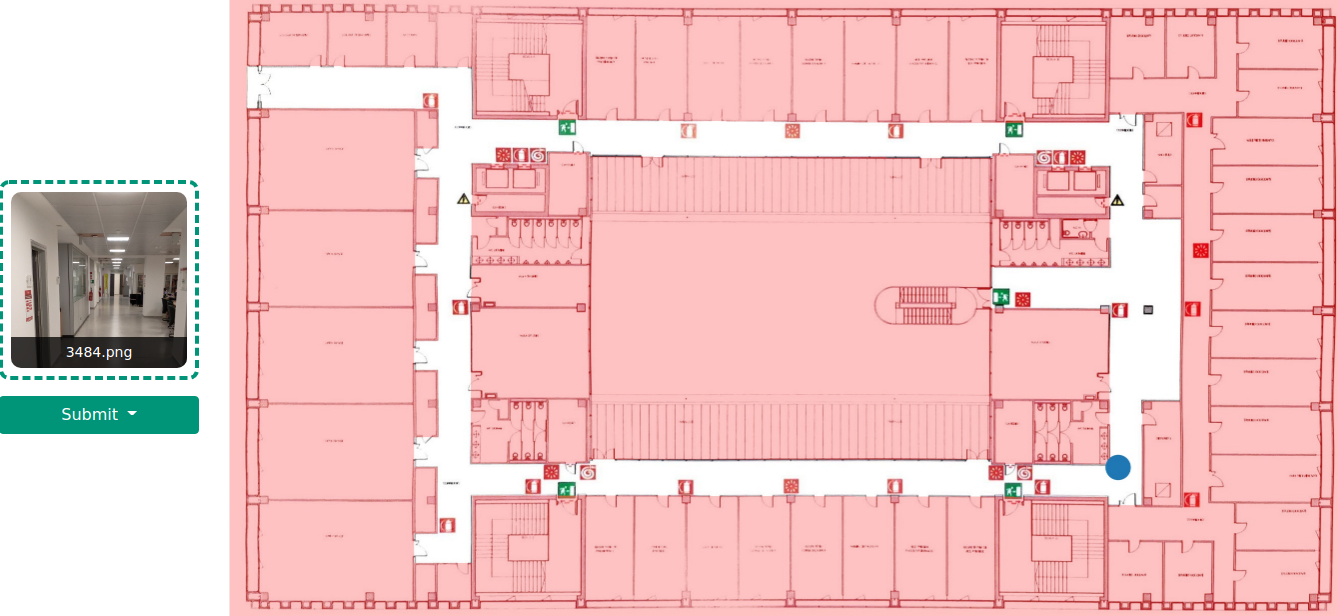
\includegraphics[width=1\textwidth]{./imgs/dashboard.png}
        \caption{Inference dashboard.}
        \label{fig:dashboard}
    \end{subfigure}
    \hfill
    \begin{subfigure}[b]{0.438\textwidth}
        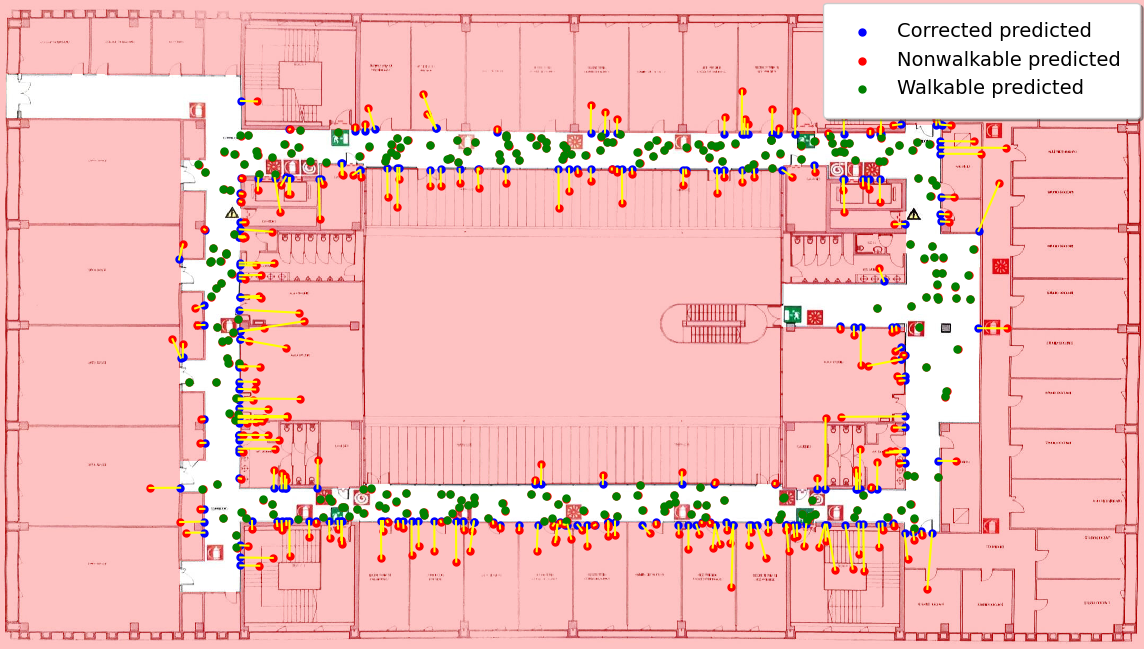
\includegraphics[width=1\textwidth]{./imgs/walkable_postprocess.png}
        \caption{Predictions post-processed on walkable areas.}
        \label{fig:trajectory-mapnet-walkable}
    \end{subfigure}
    \caption{Non walkable area maps.}
\end{figure*}
